% =========================================================================== %

\begin{frame}[t,plain]
\titlepage
\end{frame}

% =========================================================================== %

\begin{frame}{Code Quality 2}
%
\begin{columns}
\column{.3\linewidth}
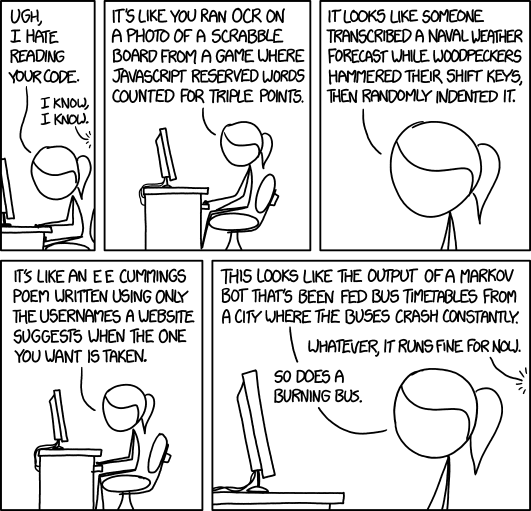
\includegraphics[width=1.3\linewidth]{./gfx/16-xkcd-code_quality_2}

\column{.4\linewidth}
\emph{It's like you tried to define a formal grammar based on fragments of a raw database dump from the QuickBooks file of a company that's about to collapse in an accounting scandal.}

\vspace{12pt}
Source: \url{https://xkcd.com/1695/}
\end{columns}
%
\end{frame}

% =========================================================================== %

\begin{frame}{Scope For Today (And Next Week)}
%
\begin{itemize}
\item Real World Application: gnuplot interface for C++
\item Disclaimer: Philosophy and Fanatism
\item SOLID Principles
	\begin{itemize}
	\item Single Responsibility Principle
	\item Open/Closed Principle
	\color{gray}
	\item Liskov Substitution Principle
	\item Interface Segregation Principle
	\item Dependency Injection Principle
	\end{itemize}
\item Some Design Patterns
	\begin{itemize}
	\item Fragments
	\item Visitor
	\end{itemize}
\end{itemize}
%
\end{frame}

% =========================================================================== %

\begin{frame}{Disclaimer: Philosophy and Fanatism}
%
\small
The guidelines presented in this lecture are largely taken from \emph{Clean Code} (Robert C. Martin).
It is certainly a worthwhile read, or, as a former fellow student once told me:

\begin{defbox}[About Clean Code]
\emph{Read it. Do it now. This is now your bible.}
\end{defbox}
\pause

This reminded me of my former physics instructor in my apprenticeship:
\begin{defbox}[About Dogmas]
\emph{Down with the slogans!}
\end{defbox}
\pause

My recommendation:
\begin{itemize}
\item Read the book. Realize that it contains more often than not good advice
\item Don't try to follow it by the word
\end{itemize}
%
\end{frame}

% =========================================================================== %

\begin{frame}[fragile]{Reoccurring Project: Gnuplot Interface for C++}
%
\begin{itemize}
\item Gnuplot: Command-Line tool to create all sorts of plots
	\begin{itemize}
	\item Simple commands entered in REPL
	\item More complex scripts in own gnuplot files
	\end{itemize}
\item Many Features
	\begin{itemize}
	\item Similar to capabilities of matplotlib
	\item Can read text- and binary files of number data
	\item Can create JPG, animated GIF, multipage-PDFs, ...
	\item Open Source, Available on Linux, Windows and MacOS
	\end{itemize}
	\pause
\item C++ Interface
	\begin{itemize}
	\item Should transform a wide range of data structures into gnuplot data files plus script
		\pause
	\item For my Master thesis: mini adaptor (v1) and a slightly more versatile library (v2)
		\begin{itemize}
		\item They did their job but were crap to use due to it not being my primary goal
		\end{itemize}
		\pause
	\item For fun, I wanted to write a \enquote{proper} version 3
		\begin{itemize}
		\item I did not abide by the SOLID principles, and the result is a (mostly usable, incomplete) mess
		\item See \url{https://github.com/TheBlueChameleon/Plotypus_3}
		\end{itemize}
		\pause
	\item Currently I'm at v4
		\begin{itemize}
		\item See \url{https://github.com/TheBlueChameleon/Plotypus_4}
		\end{itemize}
	\end{itemize}
\end{itemize}
%
\end{frame}

% =========================================================================== %

\begin{frame}{Single Responsibility Principle}
%
\begin{defbox}[Definition]
There should never be more than one reason for a class to change.
\end{defbox}
%
\begin{itemize}
\item When designing a class, try to explain its job without using the words \enquote{if}, \enquote{and}, \enquote{or}, or \enquote{but}.
\item If you can't, your class has too many responsibilities \Thus Divide
	\begin{itemize}
	\item Parallel Classes
	\item Aggregation
	\end{itemize}
\item Aim for small classes
	\begin{itemize}
	\item Use and dependencies should be grasped at a glance
	\item By extension: same principle for smaller (functions) and bigger (modules) units
	\item KISS: \emph{Keep It Simple, Stupid}
	\end{itemize}
\end{itemize}
%
\end{frame}

% =========================================================================== %

\begin{frame}{Why the SRP is Important}
%
\begin{itemize}
\item Key wording: classes should have only one reason \emph{to change}
\item Changes probably propagate
	\begin{itemize}
	\item Calls to the methods, reliance on availability of data, ...
	\item The more things a class does, the more code sites are affected when the class changes
	\item Can lead to snowball effect where a seemingly simple change requires reworking the entire code base
	\end{itemize}
\item Emergent complexity
	\begin{itemize}
	\item Interaction of very few innocent looking mechanisms can beget complex systems
	\item Complexity kills
	\end{itemize}
\item[\Thus] We want to encapsulate things into almost inert atoms
\end{itemize}
%
\end{frame}

% =========================================================================== %

\begin{frame}[fragile]{Example GnuPlot}
%
\begin{itemize}
\item User can set a \emph{terminal}
	\begin{itemize}
	\item Defines output file type (pdf, png, on screen, ...) and other properties
	\item Command \texttt{set term <terminalType> [options]}
	\end{itemize}
	\pause
\item Case PDF:
	\begin{minted}[fontsize=\scriptsize]{text}
set term pdfcairo
    {{no}enhanced} {mono|color} {font <font>} {fontscale <scale>} {linewidth <lw>} 
    {rounded|butt|square} {dashlength <dl>} {background <rgbcolor>} 
    {size <XX>{unit},<YY>{unit}}
	\end{minted}
	\pause
\item Case JPG:
	\begin{minted}[fontsize=\scriptsize]{text}
set term jpeg
    {{no}enhanced} {{no}interlace} {linewidth <lw>} {dashlength <dl>} {rounded|butt}
    {tiny | small | medium | large | giant} {font "<face> {,<pointsize>}"} 
    {fontscale <scale>} {size <x>,<y>} {{no}crop} {background <rgb_color>}
	\end{minted}
	\pause
\item And about 50 more terminal types
	\pause
\item[\Thus] Manage shared properties (\texttt{\{no\}enhanced}), unique properties (\texttt{\{no\}interlace}) and polymorphic properties (\texttt{size} with and without units)
\end{itemize}
%
\end{frame}

% =========================================================================== %

\begin{frame}{Solutions}
%
\begin{itemize}
\item Parallel Classes
	\begin{itemize}
	\item One class per terminal type
	\item Common (abstract) parent class \texttt{TerminalInfoProvider}
	\item[\Thus] Options separate, easily exchangable due to common interface
	\end{itemize}
	\pause
\item Aggregation
	\begin{itemize}
	\item Terminal Type is only one aspect of the entire project
	\item Output file names of script and generated plot file, plot types, data sources, ...
	\item[\Thus] Class \texttt{Report} \enquote{Container of class instances}
	\item[\Thus] \texttt{Report} has attributes: \texttt{TerminalInfoProvider}, \texttt{std::vector<Sheet>} (analog to \inPy{list}), ...
	\item[\Thus] \texttt{Sheet} is composed of several other classes
		\pause
	\item[\Thus] Responsibility of \texttt{Report}: Provide Infrastructure for its constituent attributes.
		\begin{itemize}
		\item E.\;g. \texttt{addSheet}
		\item E.\;g. \texttt{writeScript} -- \enquote{only} calls \texttt{writeScript} of its elements.
		\end{itemize}
	\end{itemize}
\end{itemize}
%
\end{frame}

% =========================================================================== %

\begin{frame}{New Problems and New Solutions}
%
\begin{itemize}
\item A lot of duplicate code
	\begin{itemize}
	\item Many attributes shared between different \texttt{TerminalInfoProvider}s
	\item E.\;g. \texttt{\{no\}interlace} flag
	\item Writing the attribute incl. getter and setter for each of them again and again is tedious and boring
	\end{itemize}
	\pause
\item Solution: Fragments
	\begin{itemize}
	\item Mini-Classes that only manage one property
	\item Has only attribute, getter, setter and \texttt{writeScriptFragment}
	\item Concrete \texttt{TerminalInfoProvider}s inherit from whatever Fragments they need
	\item Own package \texttt{TerminalInfoProviders} \Thus own Namespace avoids collision with other Fragments in other contexts
		\pause
	\item (Python: Inheriting same method name from multiple base classes problematic.)
		\begin{itemize}
		\item Either use \texttt{super(ClassOneBefore, self).method()}
		\item Or use aggregation: \texttt{fragments = [Fragment1(), Fragment2(), ...]}
		\end{itemize}
	\end{itemize}
\end{itemize}
%
\end{frame}

% =========================================================================== %

\begin{frame}[fragile]
%
\vspace{-5pt}
\begin{codebox}[Example: Problems with Multiple Inheritance and Solution Aggregation]
\begin{minted}[linenos, fontsize=\scriptsize]{python3}
class Base1:
    def method(self): print("Base 1")
class Base2:
    def method(self): print("Base 2")

class Derived (Base1, Base2):
    def bareSuper(self):
        super().method()               # prints only "Base 1"

    def explicitSuper(self):
        super(Derived, self).method()  # prints "Base 1"
        super(Base1, self).method()    # prints "Base 2"

class Aggregated:
    def __init__ (self):
        self.fragments = {Base1: Base1(), Base2: Base2()}

    def method(self):
        self.fragments[Base1].method()
        self.fragments[Base2].method()
\end{minted}
\end{codebox}
%
\end{frame}

% =========================================================================== %

\begin{frame}
%
\begin{recapbox}[Method Resolution Order (MRO)]
Python keeps a \inPy{list} of base \inPy{class}es for each \inPy{class}. \\
The order in this \inPy{list} determines what happens when a method is called \Thus name \emph{method resolution order}. \\
The command \inPy{super(Class, object)} translates to \emph{run on \texttt{object} with the class in the MRO \emph{after} \texttt{Class}.}

\vspace{3pt}
For some more details, see lecture 13.
\end{recapbox}
%
\end{frame}

% =========================================================================== %

\begin{frame}[fragile]{Tangent: Diamond Problem}
%
\begin{columns}
\column{.35\linewidth}
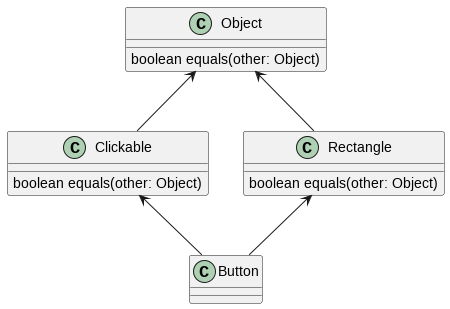
\includegraphics[width=\linewidth]{./gfx/16-uml-diamond_problem}
%
\column{.55\linewidth}
\begin{itemize}
\item Ambiguous Inheritance Situation
	\begin{itemize}
	\item \texttt{Rectangle} and \texttt{Clickable} both override \texttt{equals}
	\item \texttt{Button} does not
	\item[\Thus] What should \texttt{Button.equals} do?
	\end{itemize}
	\pause
\item Python: Depends on order in inheritance
\item C++: Requires explicit call path
\item Java: Forbids multiple inheritance ...
	\begin{itemize}
	\item ... but allows multiple interfaces with default implementations
	\item Explicit implementation (forwarding) on the lowest level (\texttt{Button}) necessary
	\end{itemize}
\end{itemize}
\end{columns}
\pause
%
\vspace{3pt}
\begin{itemize}
\item[\Thus] Avoid diamond shapes in your class graphs -- should be trees
\item[\Thus] Fragment/Aggregation pattern
\end{itemize}
%
\end{frame}

% =========================================================================== %

\begin{frame}{Project Structure Excerpt}
%
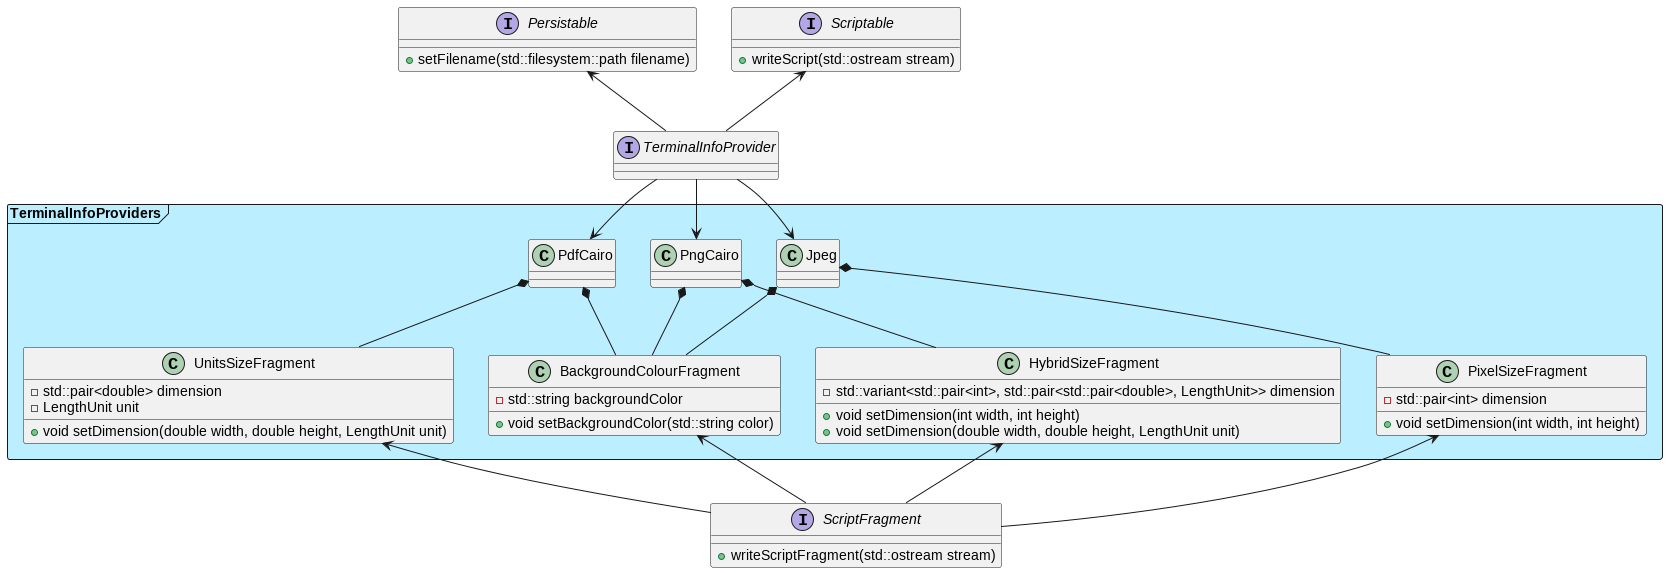
\includegraphics[width=\linewidth]{./gfx/16-uml-fragments}
%
\end{frame}

% =========================================================================== %

\begin{frame}{Controversy}
%
\begin{itemize}
\item But doesn't this give us a plethora of micro-classes?
	\pause
\item Yes, but that's not really a problem
\item You can still organize and group them in modules
\item You would otherwise have a plethora of methods, which isn't any better
\item More often than not, a simple method suddenly needs helper methods as projects grow
\item Testing becomes \emph{a lot} easier when you only need to keep one sub-scenario in mind
	\pause
\item Example from work: was \emph{encouraged to} create a new class with one method and 5 lines of code
	\pause
\item I get it if you don't like the idea, though
\item It took me a while getting used to it, too
\end{itemize}
%
\end{frame}

% =========================================================================== %

\begin{frame}{Open/Closed Principle}
%
\begin{defbox}[Definition]
Software entities (classes, modules, functions, etc.) should be open for extension, but closed for modification
\end{defbox}
%
\begin{itemize}
\item Original sense: once an entity is \enquote{done}, don't change it -- only derive.
	\begin{itemize}
	\item Classes -- by defining child classes
	\item Functions, modules -- by using wrappers
	\end{itemize}
\item Extended interpretation: Use abstract base classes to allow multiple implementations (Polymorphism)
\item[\Thus] Always keep in mind that someone (you) might use your class as a base class
\item[\Thus] Always keep in mind that someone (you) might want to replace your code in specific cases
\end{itemize}
%
\end{frame}

% =========================================================================== %

\begin{frame}{Why the OCP is Important}
%
\begin{itemize}
\item Keeping Software Closed: Similar to SRP: Avoid changes to the existing code base
	\begin{itemize}
	\item Propagating necessity to update code makes it error-prone
	\item Time consuming at the very least
	\item Binary compatibility with compiled objects may break even when functional interface is kept the same
		\begin{itemize}
		\item Less of a Python issue, but worth mentioning here
		\end{itemize}
	\item[\Thus] \emph{Never run a changing system!}
	\end{itemize}
\item Keeping Software Closed: Extensibility always desirable
	\begin{itemize}
	\item Long term future: allows re-using code in contexts not originally forseen
	\item Short term future: the currenct project may pose unforseen challenges
		\begin{itemize}
		\item For sufficiently large projects, this is the norm, not the exception
		\end{itemize}
	\item[\Thus] \emph{Don't stunt the growth of your project before you've started!}
	\end{itemize}
\end{itemize}
%
\end{frame}

% =========================================================================== %

\begin{frame}{Solutions}
%
\begin{itemize}
\item Dedicated extension attributes
	\begin{itemize}
	\item Example gnuplot interface: all classes have an optional string customOptions that is appended to the generated script
	\item Extension attribute type depends on problem at hand
	\end{itemize}
	\pause
\item Keep possibility of inheritance in mind
	\begin{itemize}
	\item Other languages: decide which attributes are private/protected or provide getters/setters
	\item Python: Use \emph{name mangling} feature (where apt) (see next slides)
	\item Write type hints and type checks such that they are open for derived classes
		\begin{itemize}
		\item E.\;g. see TypeVar and the parameter in \href{https://docs.python.org/3/library/typing.html}{\thus the documentation of the typing module}
		\item Use \inPy{isinstance(obj, ParentClass)} instead of \inPy{type(obj) == ParentClass)} 
		\end{itemize}
	\end{itemize}
	\pause
\item Provide Interfaces for Code Injection
	\begin{itemize}
	\item Example: \texttt{matplotlib.ticker.FuncFormatter}
	\item Generates texts to use as axis tick labels
	\item Initialized with a callable, takes \inPy{int, float} and returns \inPy{str}
	\item Remember: callable includes class instances with \inPy{__call__} \Thus allows arbitrary inputs beyond contractual interface
	\end{itemize}
\end{itemize}
%
\end{frame}

% =========================================================================== %

\begin{frame}[fragile]{Pseudo-Private Members and Name Mangling}
%
\begin{itemize}
\item Private Members:
	\begin{itemize}
	\item Concept of many OO languages: access only from within class methods
	\item Prevents inconsistent state by limiting the ways mutation can happen (\thus only via methods guaranteed to generate a valid state)
	\item Help with inheritance: derived class can't see private members, hence may define members of the same name
	\end{itemize}
	\pause
\item Protected Members:
	\begin{itemize}
	\item Refinement of concept private members
	\item Accessible from within class \emph{and derived classes}, but not from outside
	\end{itemize}
	\pause
\item Python: no such concept
	\begin{itemize}
	\item Convention: treat members beginning with a single underscore as private
	\item Name mangling when beginning with a double underscore:
		\begin{itemize}
		\item \texttt{\_\_foo} automatically becomes \texttt{\_TheClass\_\_foo}
		\item Avoids (most) name clashes
		\item You can still \texttt{instance.\_TheClass\_\_foo}
		\end{itemize}
	\end{itemize}
\end{itemize}
%
\end{frame}

% =========================================================================== %

\begin{frame}[fragile]
%
\begin{codebox}[Name Mangling]
\begin{minted}[linenos, fontsize=\scriptsize]{python3}
class Foo:
    def __init__(self):
        self.__private_member = None

    def __private_function(self):
        pass

instance = Foo()
print(dir(instance))
\end{minted}
\end{codebox}
%
\begin{cmdbox}[Output]
\begin{minted}[fontsize=\scriptsize]{text}
['_Foo__private_function', '_Foo__private_member', '__class__', '__delattr__',
 '__dict__', '__dir__', '__doc__', '__eq__', '__format__', '__ge__',
 '__getattribute__', '__getstate__', '__gt__', '__hash__', '__init__',
 '__init_subclass__', '__le__', '__lt__', '__module__', '__ne__', '__new__',
 '__reduce__', '__reduce_ex__', '__repr__', '__setattr__', '__sizeof__',
 '__str__', '__subclasshook__', '__weakref__']
\end{minted}
\end{cmdbox}
%
\end{frame}

% =========================================================================== %

\begin{frame}[fragile]
%
\vspace*{-7pt}
\begin{defbox}[Tangent: On why there are no private members in Python]
\footnotesize
\enquote{\emph{{\color{gray}No, it means that} in Python we are consenting adults, and either respect
attributes with a leading underscore as private - or willfully chose to
*not* do that because of good reasons.}}

\vspace{3pt}
Quote from \href{https://mail.python.org/pipermail/python-list/2009-November.txt}{\thus The Python Mailing List}
\end{defbox}
%
\vspace*{-10pt}
\begin{codebox}[Privacy vs Dynamicity]
\begin{minted}[linenos, fontsize=\scriptsize]{python3}
def method(obj, recurse=False):
    obj.member = "something"
    if recurse: method(self, False)
    
class Foo:
    def __init__(self):
        self.member = None

Foo.method = method

foo = Foo()
foo.method()
method(foo)
\end{minted}
\end{codebox}
%
\end{frame}

% =========================================================================== %

\begin{frame}
%
\begin{hintbox}[Don't Overdo It]
While it's not wrong to use the name mangling feature for every attribute, you'll find it cumbersome soon enough.

\vspace{3pt}
The extra effort is not really needed that often. A user that inherits from your class will work in the same context, \ie they'd most likely pick the same name for the same concept.
Only where words are ambiguous, this extra safety measure may prove worth the hassle.

\vspace{3pt}
Also, not all classes are automatically likely to be derived from by users.
Usually only such classes that are accepted as parameters to other methods of your project need to be taken care of.
\end{hintbox}
%
\end{frame}

% =========================================================================== %

\begin{frame}{Example GnuPlot}
%
\begin{itemize}
\item Simple line plot:\\
	\begin{itemize}
	\item Assume there is a tab-separated file \texttt{numbers.dat} with the x values in the first and the y values in the third column
	\item \texttt{plot 'numbers.dat' using 1:3 with lines}
	\item You can also omit the x values (automatically uses the numbers $1, 2, ... N$ as x values)
	\end{itemize}
	\pause
\item 3D line plot:\\
	\begin{itemize}
	\item Assume there \texttt{numbers.dat} has x, y, z in first, second, third column
	\item \texttt{{\color{blue}s}plot 'numbers.dat' using 1:2:3 with lines}
	\item[\Thus] Tempting to retrofit a parameter \texttt{is3D} that adds the \texttt{s} and allows an extra input column
		\pause
	\item ... but on the same plot there may only be 2D \emph{or} 3D plots
	\item ... and the configuration of axes is different
	\item ... and in other plot types, this gives much more variation
	\end{itemize}
	\pause
\item[\Thus] Forcing 3D capabilities on a single \texttt{Plot} class is aksing for trouble
	\pause
\item[\Thus] Rather make a separate Plot2D and a Plot3D class
	\begin{itemize}
	\item It turns out, pie charts also need special treatment, so it's well worth the effort
	\end{itemize}
\end{itemize}
%
\end{frame}

% =========================================================================== %

\begin{frame}
%
\begin{recapbox}[Iteratables and Iterators]
An \emph{Iterable} is any structure you can \emph{iterate} over, \ie put it into a \inPy{for} statement (\inPy{for element in myIterable}). Examples include Python's \inPy{list}, \inPy{set}, \inPy{dict}, etc. User-defined structures can also be made into iterables.\\
The defining characteristic of an iterable is that it has a \inPy{__iter__} method which returns an \emph{Iterator}.

\vspace{3pt}
An \emph{Iterable} is a book keeping device that stores which element is next in the iteration. This can be in the form of a simple index variable for a list, or a more complex aggregate of information, for example when iterating over a tree structure.\\
The defining characteristic of an iterable is that it has a \inPy{__next__} method which returns the next element for the \inPy{for} loop.

\vspace{3pt}
For some more details, see lecture 3.
\end{recapbox}
%
\end{frame}

% =========================================================================== %

\begin{frame}{Visitor Pattern and Double Dispatch}
%
\begin{itemize}
\item Given
	\begin{itemize}
	\item Hierarchical structure of objects and subobjects of different types
	\item I.\;e. several \inPy{class}es with multiple instances each, related to each other
	\item Well defined iterator over the structure
	\item Example: file system: tree of files and directories
	\end{itemize}
\item Want
	\begin{itemize}
	\item One or more operations that touch each element exactly once
	\item Examples: show indented list on screen; pack into .zip archive
	\end{itemize}
\item Problems
	\begin{itemize}
	\item Polymorphic structure -- elements require different treatment depending on their type
	\item Original classes might be considered closed
	\end{itemize}
\end{itemize}
%
\end{frame}

% =========================================================================== %

\begin{frame}{Solution Part 1: Visitor Pattern}
%
\begin{itemize}
\item Put the operations into a Visitor class
	\begin{itemize}
	\item Visitor class has methods like \texttt{doFor<Type>(element)}
	\item Often, for convenience: method \texttt{traverse(rootElement)}
	\end{itemize}
\item[\Thus] Functionality Extended without any changes to the original classes
\item[\Thus] Repeatable (more features can be added in the same way)
\item[\Thus] Single Responsibility Principle obeyed!
\pause
\end{itemize}

\vspace{6pt}
... but how should \texttt{traverse} choose, which \texttt{doFor} method should be called?
\begin{itemize}
\item Naive approach: type checking
	\begin{itemize}
	\item \inPy{if isinstance(element, SomeType): doForSomeType(element)}
	\item Problem: Requires update of \texttt{traverse} method whenever new types are introduced
	\item Problem: May lead to ambiguous situations when there are derived classes
	\end{itemize}
\end{itemize}
%
\end{frame}

% =========================================================================== %

\begin{frame}{Solution Part 2: Double Dispatch}
%
\begin{itemize}
\item \emph{Dispatching}: send off to a destination or for a purpose.
\item In context of the pattern:
	\begin{itemize}
	\item Visitor calls a function \texttt{accept(visitor)} of the target class (\thus first dispatch)
	\item Method \texttt{accept} calls the proper \texttt{doFor<Type>} method of \texttt{visitor} (because the class obviously knows its own type)
	\end{itemize}
\pause
\item Requires change to the original classes, but ...
	\begin{itemize}
	\item ... at least a trivial one
	\item ... can still be attached to strictly closed classes by inheritance (\texttt{Type} \thus \texttt{VisitableType})
	\end{itemize}
\item Introduces some coupling between \texttt{Type} classes and their \texttt{Visitor}(s)
	\begin{itemize}
	\item Common name scheme for the \texttt{doFor<Type>} methods
	\item Can be enforced with abstract interface of the Visitor (\texttt{ZipPacker} inherits from \texttt{FileVisitor} and \texttt{DirectoryVisitor})
	\end{itemize}
\end{itemize}
%
\end{frame}

% =========================================================================== %

\begin{frame}{Some Remarks On When To Use All Of This}
%
\begin{itemize}
\item We've seen that these principles force us to introduce a lot of extra classes
\item This \emph{does} add boilerplate code and extra work
\item Certainly not necessary in small, \enquote{disposable} single-purpose scripts
	\begin{itemize}
	\item 90\% of what I do in Python falls in this category ...
	\item ... but that's a matter of personal taste
	\end{itemize}
\pause
\item The more complex projects become, the more valuable these principles become
	\begin{itemize}
	\item Projects are always more complex than they seem at the start
	\item Desire to expand on finished projects arises very often
	\item Most of my failed projects can be attributed to raising complexity up to the point where I couldn't handle the interconnectedness any longer
	\end{itemize}
\pause
\item[\Thus] If you aren't going to finish your code on the same day: follow the guidelines
\end{itemize}
%
\end{frame}

% =========================================================================== %